%\begin{frame}
%\frametitle{Massless particles and helicity}
%\begin{columns}
%\column{0.5\textwidth}
%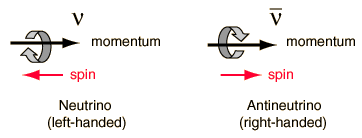
\includegraphics[scale=0.35]{img/NeutrinoHelicity.png}
%
%Helicity is the spin projection in the direction of motion.
%\[
%h = \frac{\va{\sigma}\cdot \va{p}}{p}
%\]
%In the limit of $m \rightarrow 0$~ Dirac's equation(s) decouple in 
%two states with definite helicity:
% \begin{empheq}[box=\fbox]{align}
%(E +  \va{p}\cdot\va{\sigma}) \chi  & = 0 \nonumber \\
%(E -  \va{p}\cdot\va{\sigma}) \phi  & = 0 \nonumber
%\end{empheq}
%The particle has negative helicity and the antiparticle positive helicity. \alert{Massless particles have well defined helicity}. \column{0.5\textwidth}
%
%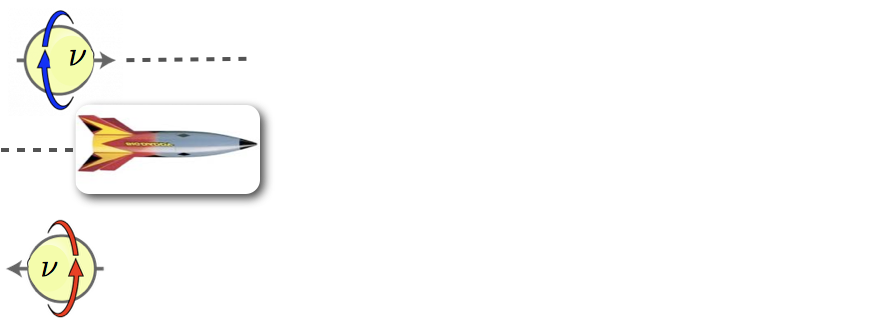
\includegraphics[scale=0.30]{img/neutrinoBoost2.png}
%
%For massive particles, helicity depends on the reference frame. One can always jump into a reference system faster than that of the particle and see its helicity flip.
%
%But massless particles travel at the speed of light and cannot be overtaken. The helicity becomes a constant of motion. 
%\end{columns}
%
%\end{frame}
%
%\begin{frame}
%\frametitle{Neutrino oscillations}
%%\begin{columns}
%%\column{0.4\textwidth}
%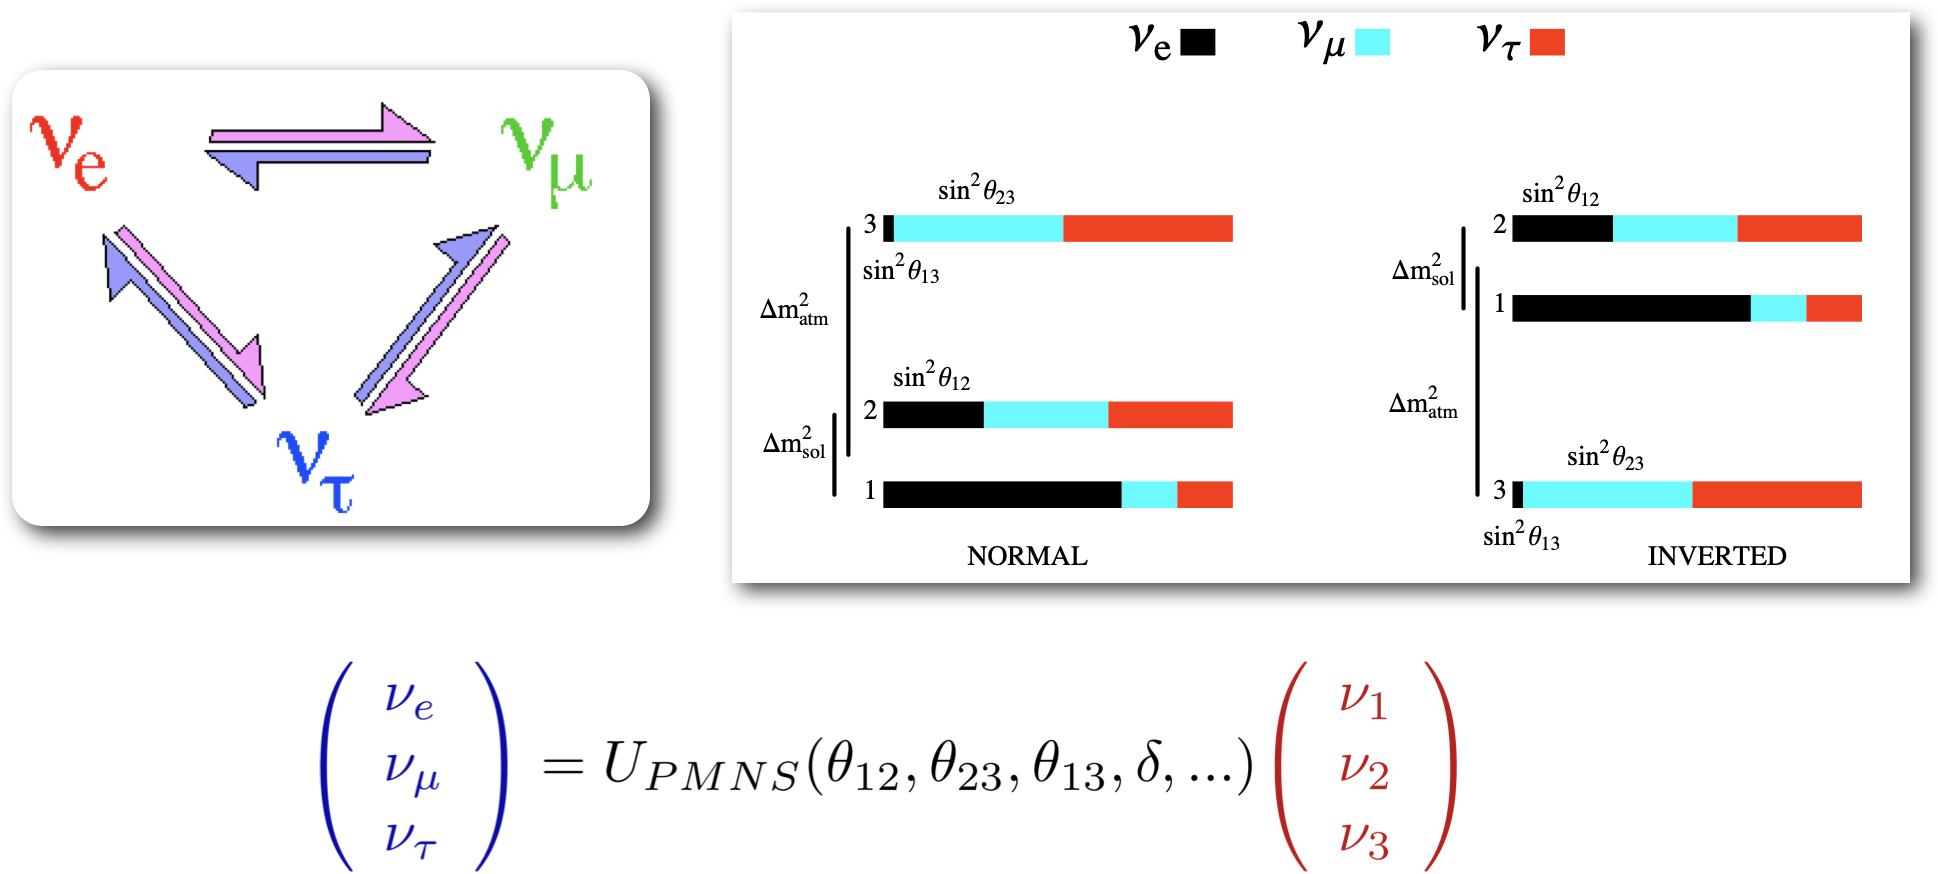
\includegraphics[scale=0.30]{img/neutrinoOscillations.png}
%%\column{0.4\textwidth}
%%\begin{block}{}
%
%Neutrino oscillation experiments (a story to be told some other time) have established that neutrinos are massive. Their mass is, however, very small. This is the reason why parity experiments found the neutrino to be left handed, since the effects associated to their masses are of the order of $m/E$~where $m$~is the mass of the neutrino (tiny) and $E$~the energy of the process (much larger). 
%
%\alert{But how do we give a mass to the neutrinos?} 
%
%%\end{block}
%%\end{columns}
%\end{frame}
%
%\begin{frame}
%\frametitle{Electron mass}
%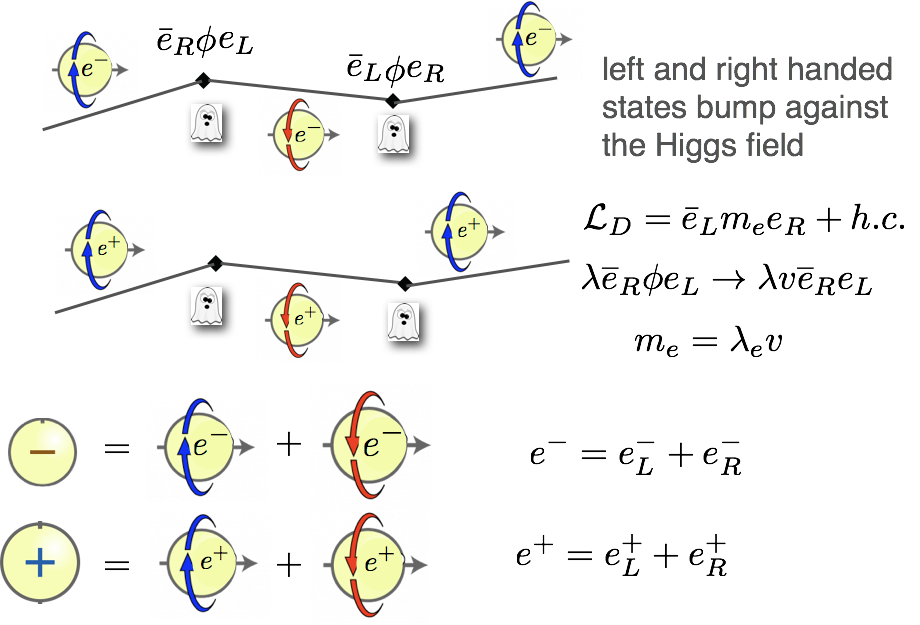
\includegraphics[scale=0.30]{img/ElectronMass.png}
%\end{frame}

\begin{frame}
\frametitle{Neutrino mass (Dirac recipe)}
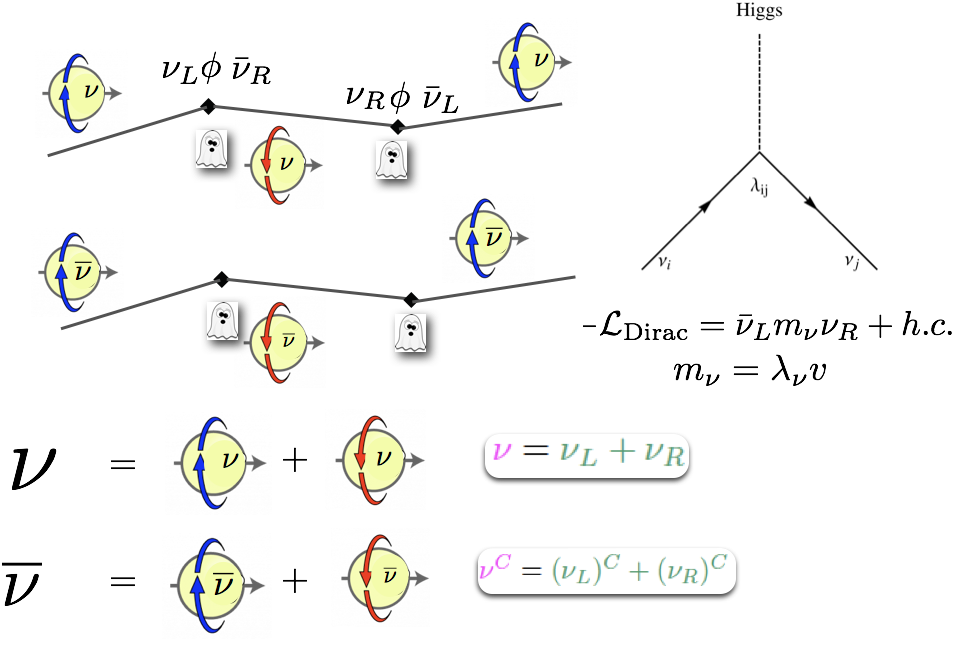
\includegraphics[scale=0.30]{img/NeutrinoMassDirac.png}
\end{frame}

\begin{frame}
\frametitle{Deus ex machina}
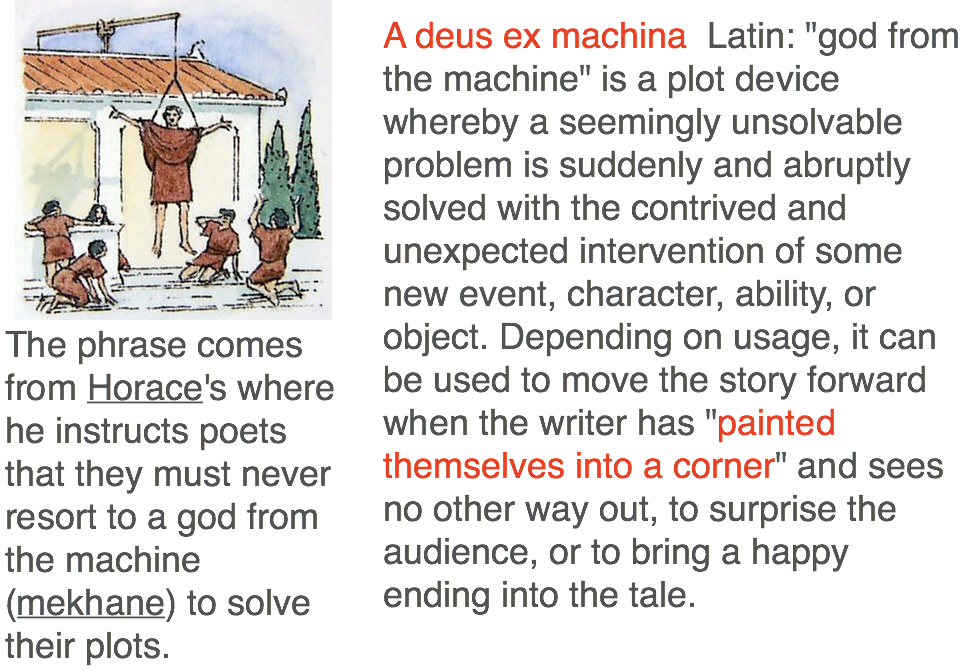
\includegraphics[scale=0.30]{img/DeusExMachina.png}
\end{frame}

\begin{frame}
\frametitle{Dirac neutrino mass: Deus ex machina}
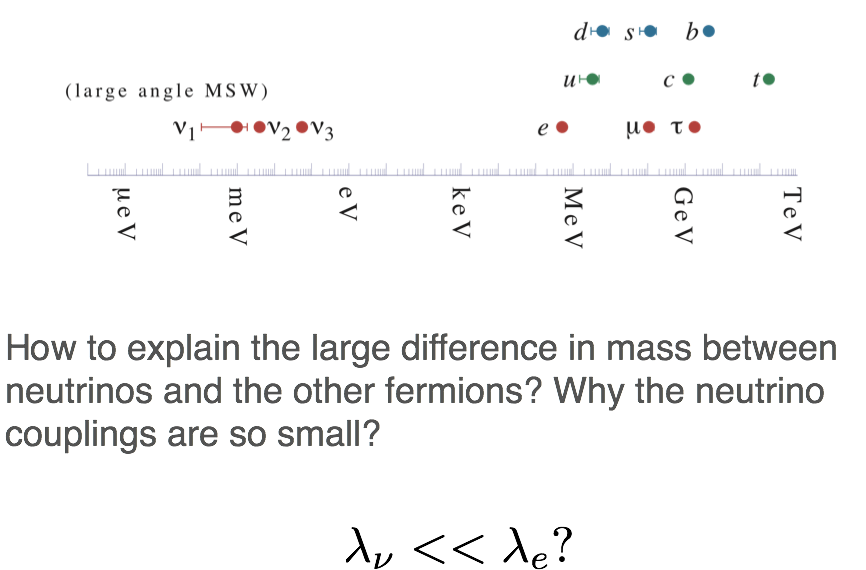
\includegraphics[scale=0.30]{img/SmallNeutrinoMasses.png}
\end{frame}

\begin{frame}
\frametitle{Majorana neutrinos}
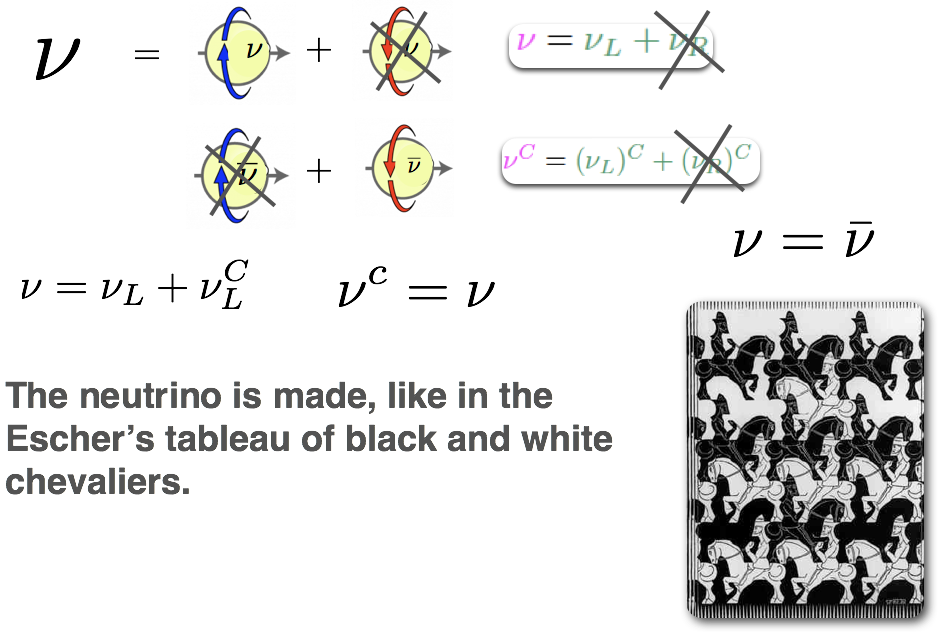
\includegraphics[scale=0.30]{img/MajoranaNeutrinosCartoon.png}
\end{frame}

\begin{frame}
\frametitle{Majorana mass}
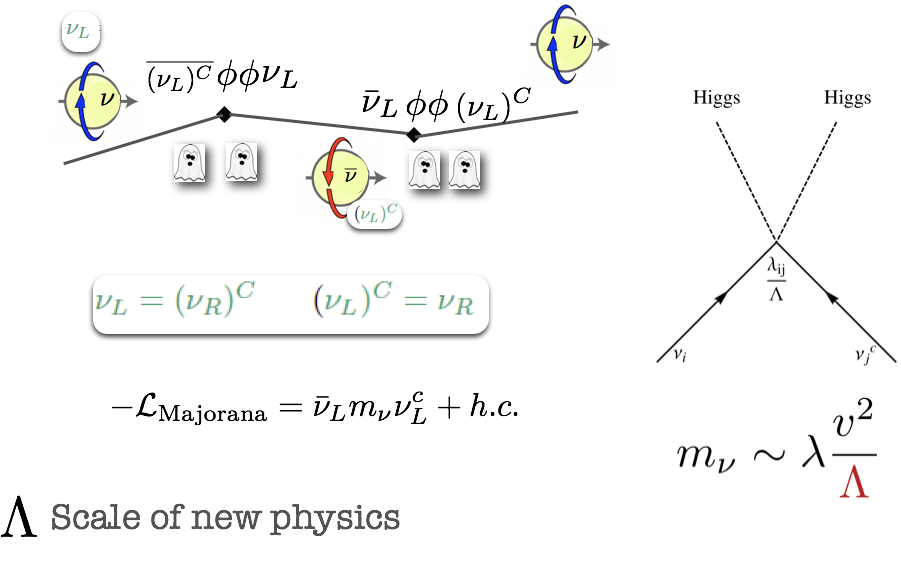
\includegraphics[scale=0.30]{img/MajoranaMass.png}
\end{frame}

\begin{frame}
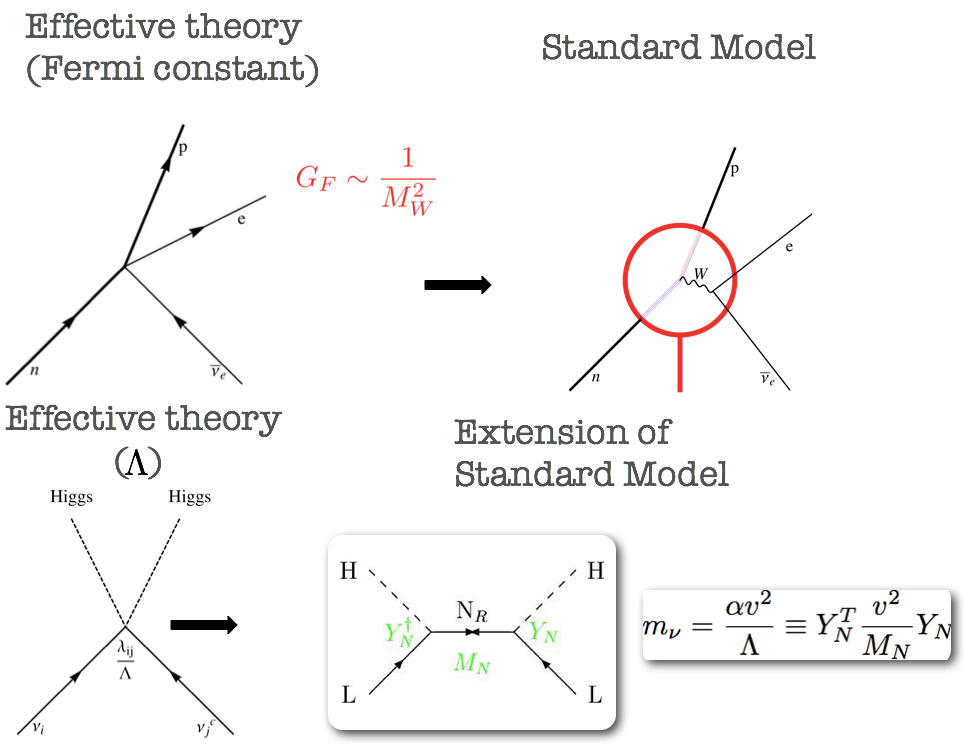
\includegraphics[scale=0.30]{img/Effective.png}
\end{frame}

\begin{frame}
\frametitle{The mystery of the missing antimatter}
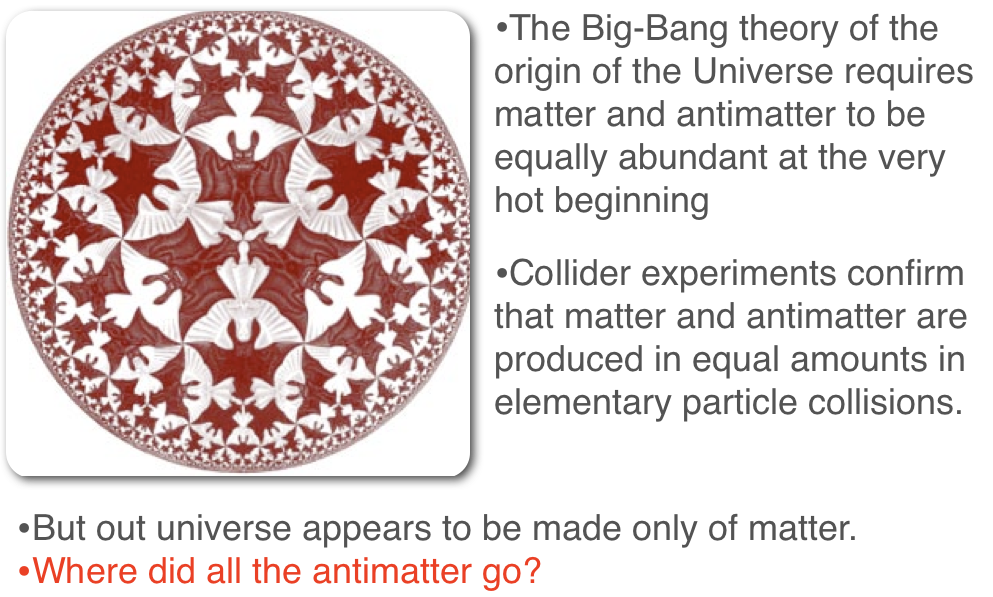
\includegraphics[scale=0.30]{img/MissingAntiMatter.png}
\end{frame}

\begin{frame}
\frametitle{CP violation and Majorana neutrinos}
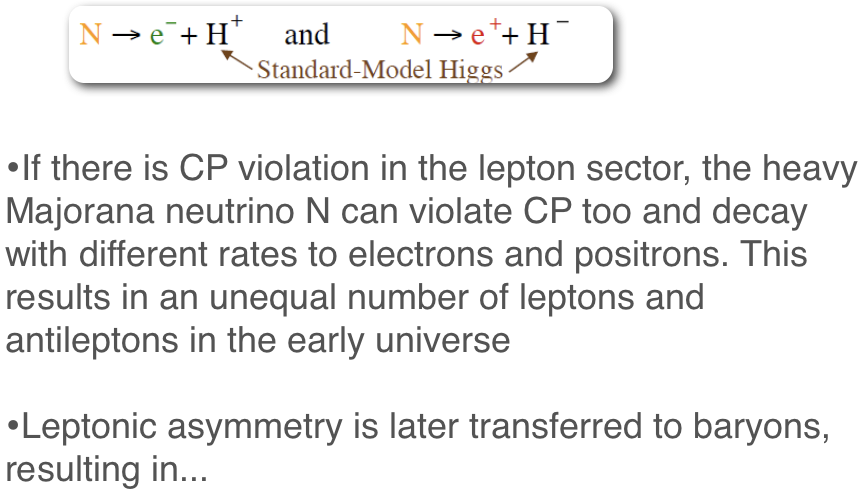
\includegraphics[scale=0.30]{img/CP.png}
\end{frame}

\begin{frame}
\frametitle{We are the leftovers}
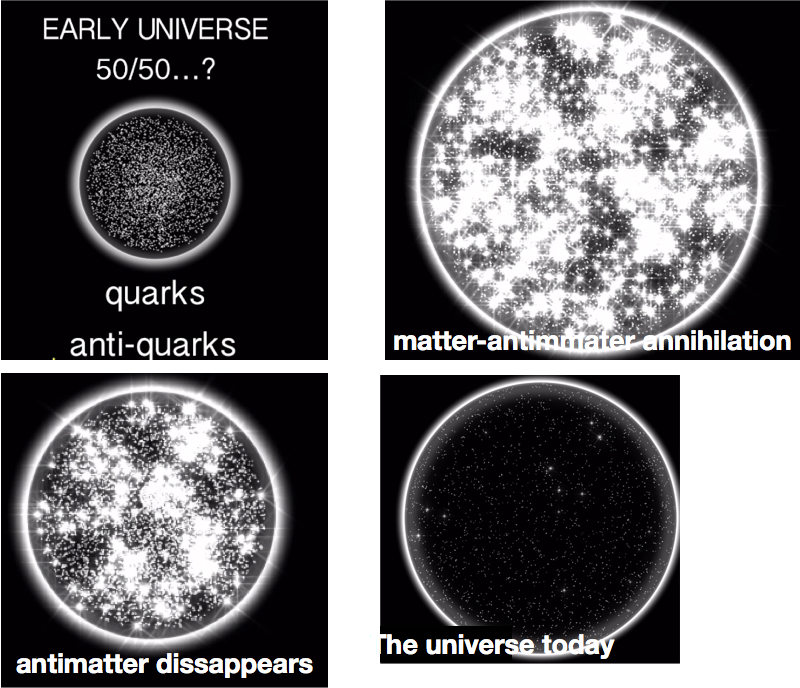
\includegraphics[scale=0.30]{img/MissingUniverse.png}
\end{frame}
%

\begin{frame}
\frametitle{A formula for the Universe}
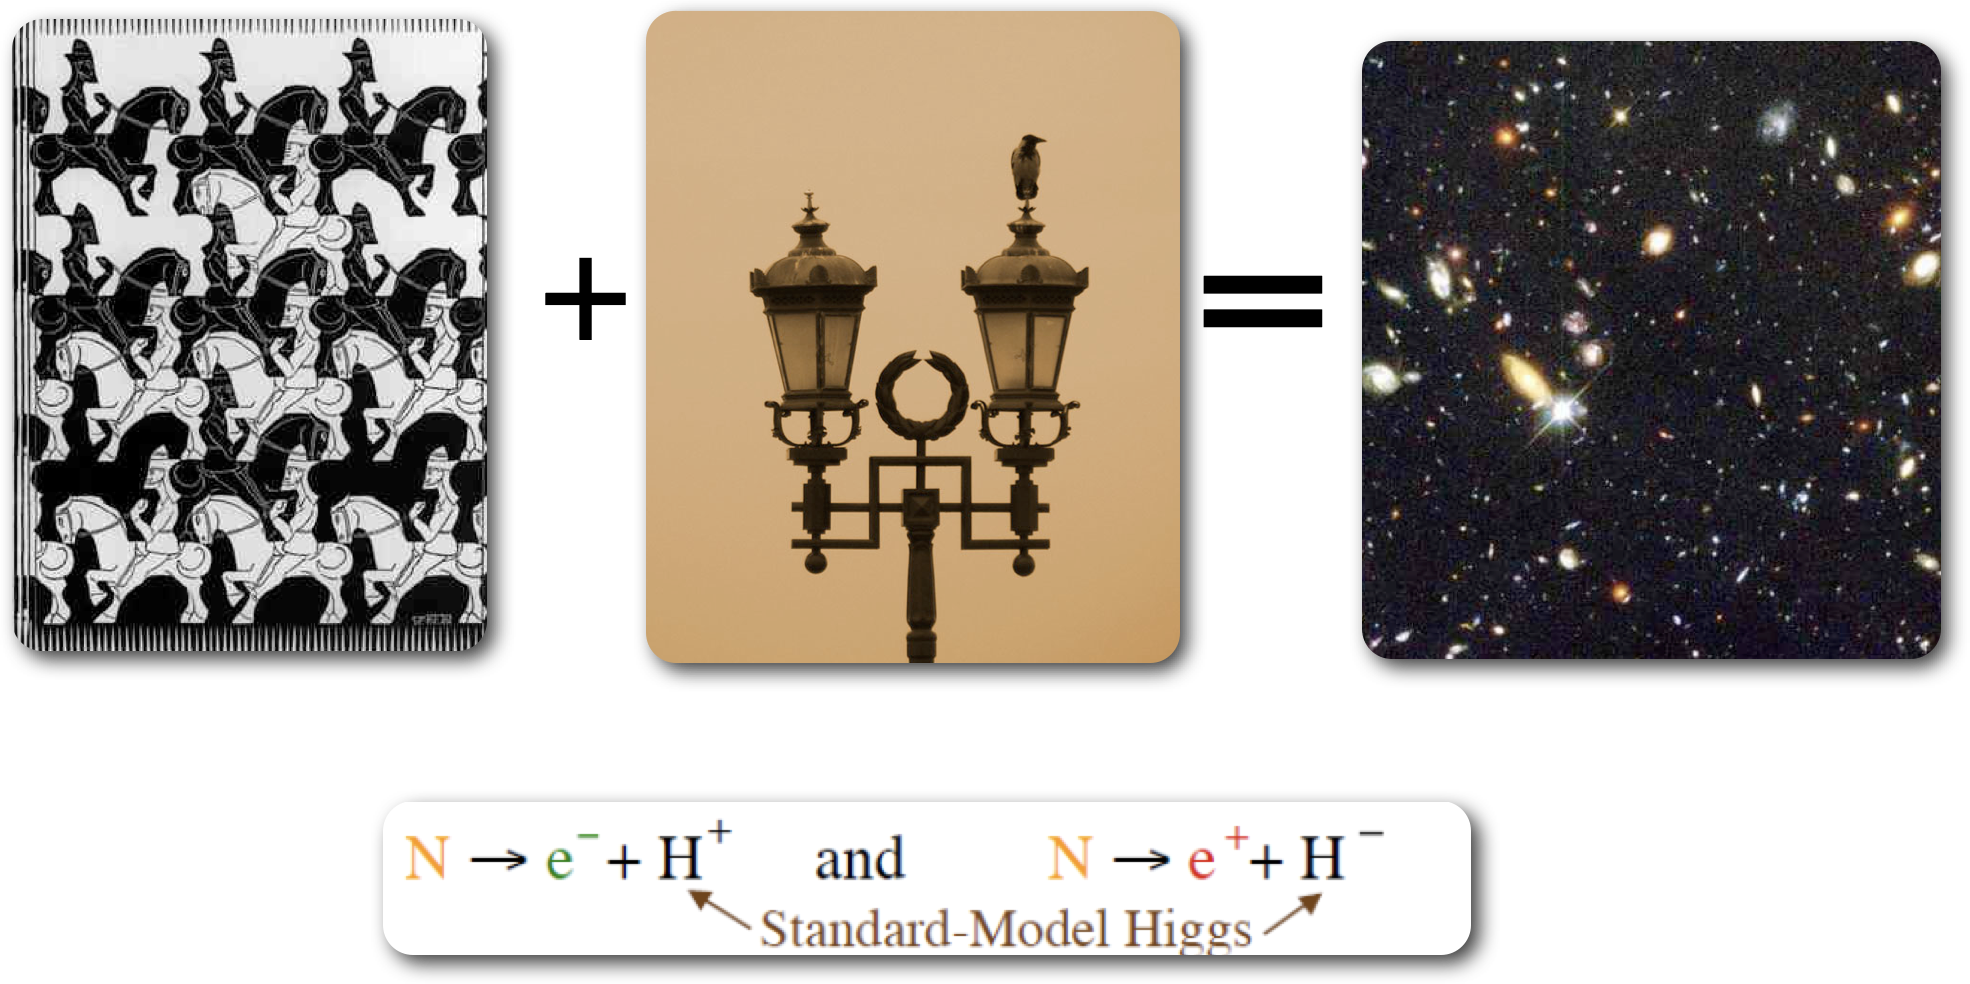
\includegraphics[scale=0.30]{img/formulaUniverse.png}
\end{frame}









